\chapter{Results}
\label{ch:Results}
% Do not write long version of imu or lidar acronym again
\glslocalunset{imu}
\glslocalunset{lidar}

\section{Evaluation concept}
During each test drive the measurements of the accelerometer and gyroscope of the \gls{imu} (of both \glspl{imu}, myAHRS+ and of the \gls{imu} integrated in the ZED 2i camera), the camera image of the ZED 2i camera and the point cloud generated by the \gls{lidar} are recorded.
Only one \gls{lidar} could be mounted at a time, so the Velodyne UltraPuck was used for most test drives, but two recordings were also made using the Robosense.
Furthermore, the wheel speeds were recorded when available, which was only the case when driving a ramp down or only half-way up, as mentioned in \cref{sec:car}.\\
To prevent an overfitting of the model it is important to have different test scenarios.
As mentioned in \cref{sec:garage}, four different ramps were available to test the model.
For the evaluation of the \gls{imu} only the ramps A B, and D will be used.
Multiple test drives were made for each scenario, the most drives where performed on ramp A.
Because the wheel speed sensor measurements are needed for some methods, which are only available in a special mode where the power of the car is very limited, the ramps A and B could only be driven halfway up.
But a full recording including the wheel speed measurements could be done for ramp D and A, when driving down.\\
The \gls{lidar} and camera only detect ramps going up, so only the ramps A, B and C were used.
Furthermore, a test drive without any ramps in sight was made to test if false positives are being detected.



\section{Reference data}
To evaluate the performance of the different algorithms a reference is necessary.
The open-source \gls{ros} package \texttt{hdl\_graph\_slam}~\footnote{\url{https://github.com/koide3/hdl_graph_slam}} is used for this task.
It is based on 3D graph \gls{slam} and uses the \gls{lidar} data to map the environment and estimate the pose (position and orientation) of the car.
It uses NDT scan matching-based odometry estimation with loop detection.
The point cloud of common features at time $t$ is compared to the point cloud from the time $t-1$ and matched against each other.
The algorithm then estimates the translation and orientation difference between those two point clouds.
In ref.~\cite{Akpnar2021} the accuracy of the HDL Graph \gls{slam} was tested and a mean error of \SI{4}{\cm} and a standard deviation of \SI{5}{\cm} was measured for an indoor scenario.\\
From the pose information of the HDL Graph \gls{slam} the pitch angle of the car can be calculated and be used as a reference for the road grade, to evaluate the performance of the different \gls{imu}-based methods.
Because the \gls{lidar} only records at \SI{10}{\hertz} and thus the estimation of the HDL Graph \gls{slam} also only updates at \SI{10}{\hertz}, but the other sensors record from \SIrange{100}{400}{\hertz}, the estimate was upsampled using a Fourier method.
Beside estimating the road grade, the \gls{imu} is used to estimate the angle and length of the ramp.
Both of those values can be extracted from the generated point cloud map, by measuring the distance between the corresponding points.
Because the ramp angle is not constant, the average angle of the ramp is used as reference.
The average angle $\alpha$ is calculated by measuring the length and height of the ramp and using the law of sines
\begin{equation}
	\alpha = \arcsin\left(\frac{h_\mathrm{ramp}}{l_\mathrm{ramp}}\right).
\end{equation}
The \gls{lidar} is used to detect and track the distance to the ramp and also to estimate the width and angle.
For the evaluation of the tracking accuracy, the generated map and pose provided by the HDL Graph \gls{slam} is used again.
In the generated point cloud map, the ramp region was marked manually by visual inspection.
Then using the position of the car, provided by the \gls{slam}, the true distance to the beginning of the ramp could be calculated, by measuring the distance of the current position to the beginning of the ramp for each frame.\\
An example of the point cloud map generated by the \texttt{hdl\_graph\_slam} package is shown in \cref{fig:pcd_rviz}.
The color of the points gives information about the z-value (height information) of the points.
The ramp region is marked by the bigger points and the white arrows visualize the trajectory of the car.
In this example the car was driven only half-way up the ramp.
\begin{figure}[htbp]
	\centering
	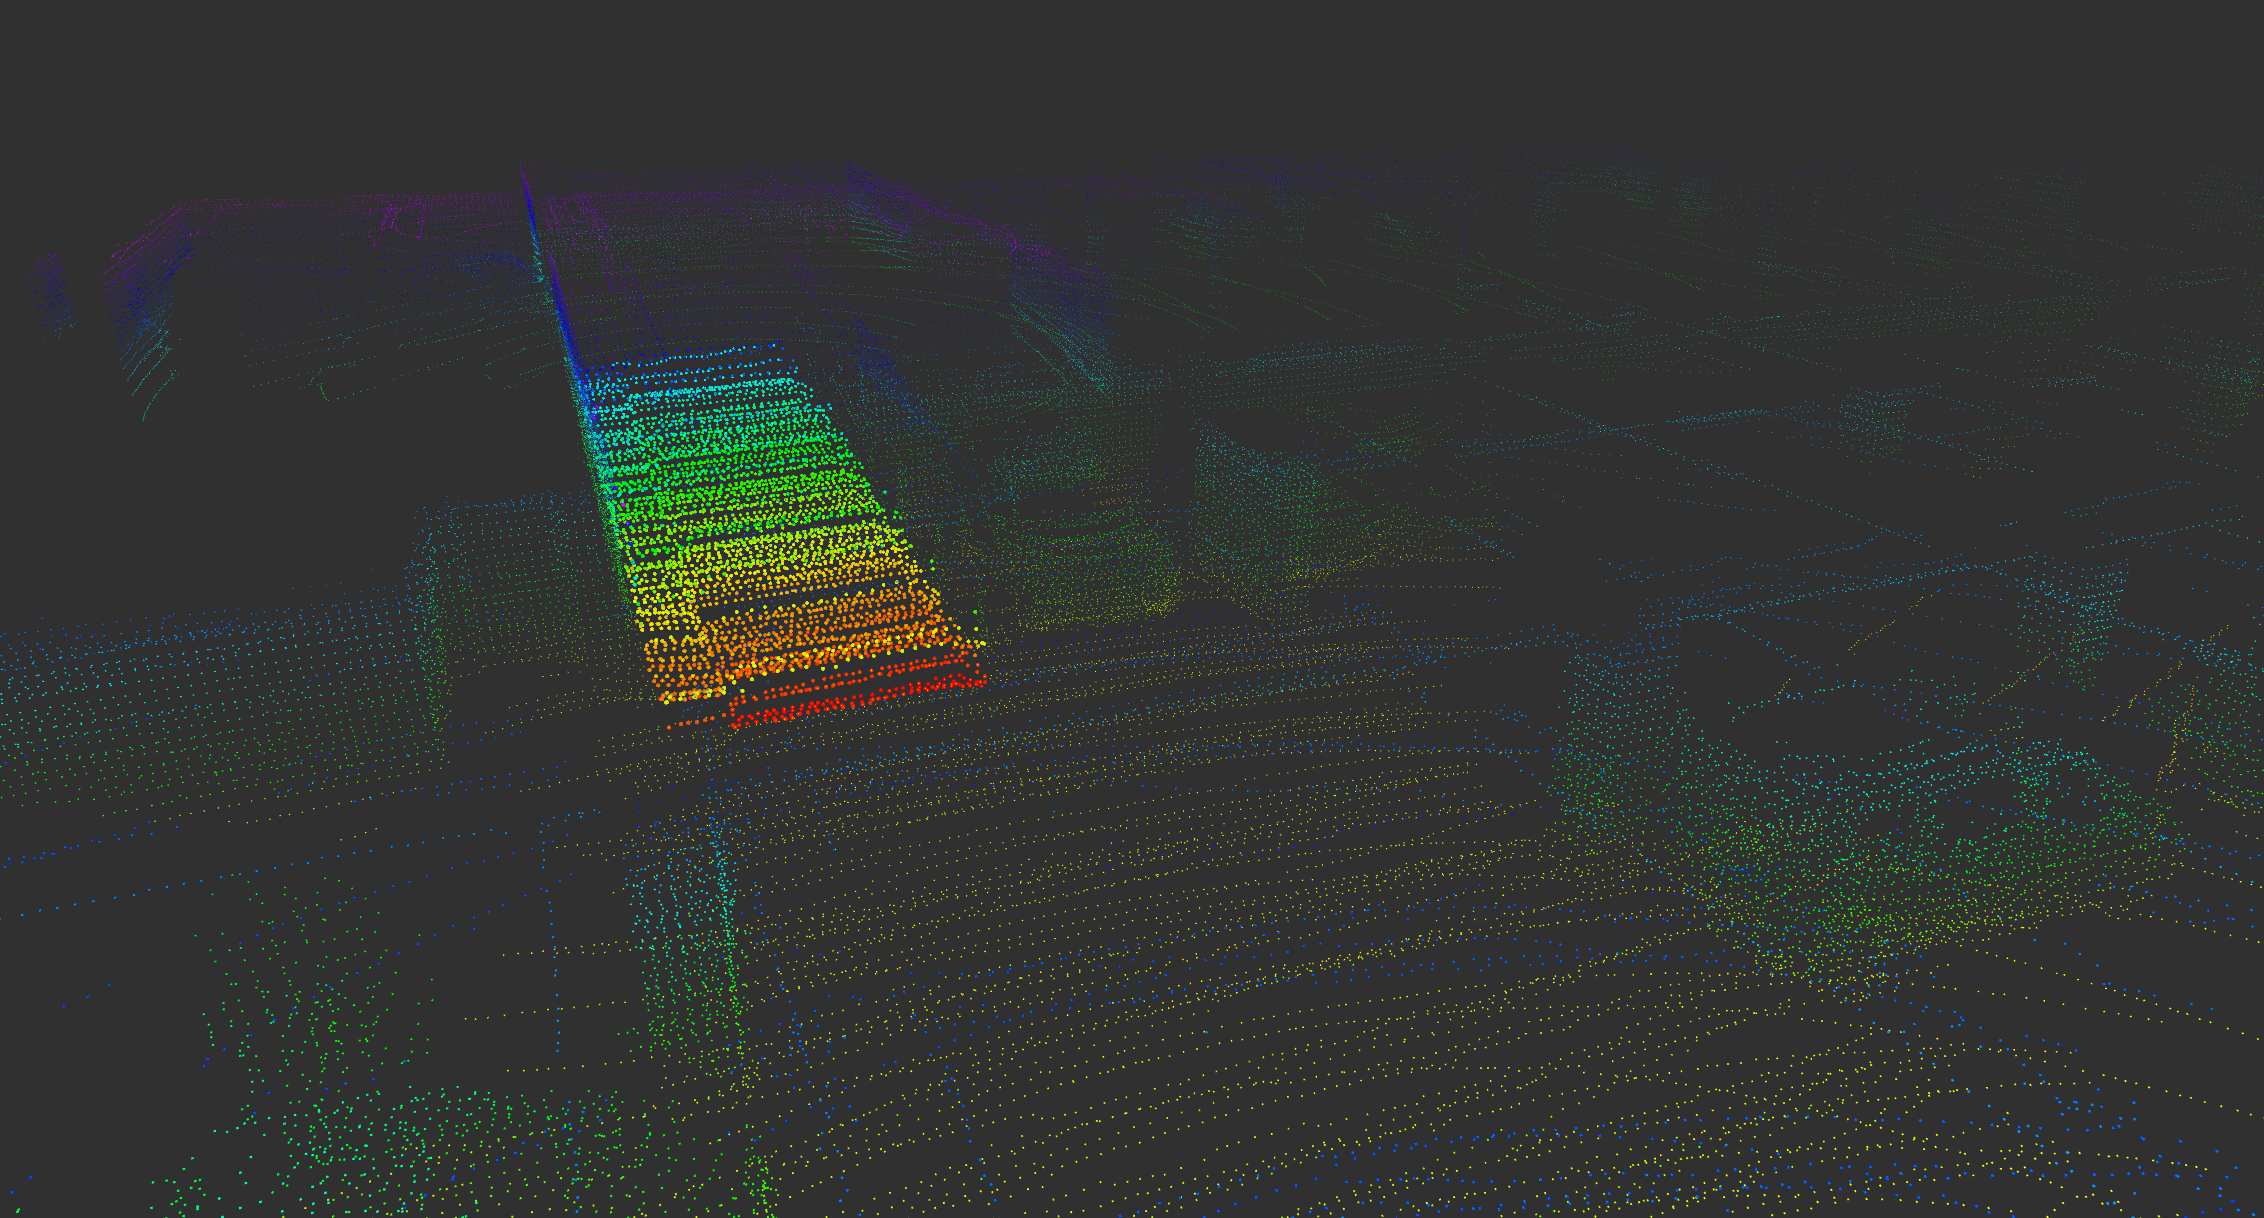
\includegraphics[width=.9\linewidth]{pcd_rviz.png}
	\caption[Generated point cloud]{The by the \texttt{hdl\_graph\_slam} package generated point cloud map. The white arrows visualize the trajectory of the car.}
	\label{fig:pcd_rviz}
\end{figure}



\section{Performance measures}
\iimprov{Probably change \gls{rmse} to st dev for constant reference}
In order to ...
the following \gls{kpi} are used.
The goodness of the fit between the estimated road grade $\hat{y} = (\hat{y}_i, \dots, \hat{y}_n)^\intercal$ and the reference $y = (y_i, \dots, y_n)^\intercal$ can be described by the \gls{rmse}
\begin{equation}
	RMSE = \sqrt{\frac{1}{n}\sum_{i = 1}^n(\hat{y}_i - y_i)^2},
\end{equation}
which quantifies how much the predicted values differ from the reference value on average.
It is defined in the range $[0, \infty)$, with a value of 0 indicating a perfect fit.
Furthermore, the coefficient of determination $R^2$ is used
\begin{equation}
	R^2 = 1 - \frac{\sum\limits_{i = 1}^n(\hat{y}_i - y_i)^2}{\sum\limits_{i = 1}^n(\hat{y}_i - \overline{y})^2},
\end{equation}
where $\overline{y}$ indicates the mean of the reference.
The goodness of the fit is described in the range from 0 to 1, where 1 describes a perfect fit.\\



\section{Ramp metering? (\glsentryshort{imu})}
\begin{figure}[htbp]
	\centering
	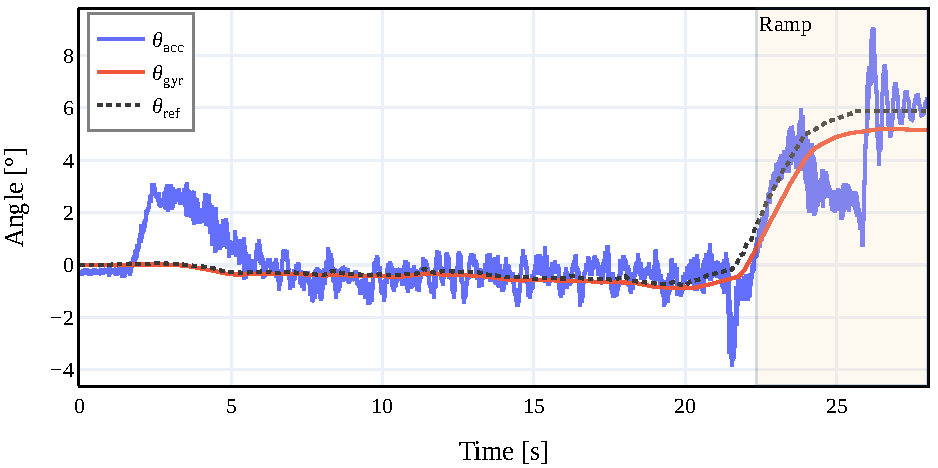
\includegraphics[width=.9\linewidth]{imu_raw_angle.pdf}
	\caption[Raw]{Pitch angle estimation from the raw accelerometer and gyroscope measurements}
	\label{fig:imu_raw_angle}
\end{figure}
Different recordings of different ramps were made, but the results will be discussed on only two test drives.
Furthermore, two different \glspl{imu} were used, but only the measurements of the ZED 2i \gls{imu} will be used, due to being more precise.
The difference between the two sensors can be seen in
\itodo{Either add graph showing performance of both imus or ref to table}
In the first drive the car was accelerated from stand still and drove up ramp A about half-way up.
As explained in \cref{sec:car}, the ramp could not be driven completely, due to the need of the odometer readings, which are only available when the motor output is limited.
\subsection{Road grade estimation}
The ramp detection using the \gls{imu} relies on the correct estimation of the road grade angle.
Hence, the evaluation of the goodness of the estimation is necessary to determine the performance of the ramp detection algorithm.\\
The result of using only the raw measurements of the \gls{imu} for the pitch calculation is shown in \cref{fig:imu_raw_angle}.
The measurement by the accelerometer is very noisy and is easily influenced by accelerations other than gravity, which can be seen at \SIrange{2}{4}{\second}, where the car started driving.
The gyroscope on the other hand provides good short-term accuracy and is not influenced by other accelerations, but is slowly drifting over time.
The time frame during which the car was on the ramp is marked by the yellow coloring.
The start of the ramp is being defined, when the reference data surpasses \ang{1.5}.\\
The gravity method tries to overcome the problem of the accelerometer of also detecting other accelerations than gravity, by subtracting the car's acceleration from the accelerometer measurement.
The car's acceleration $\vb{a}_\mathrm{odom,x} $ was calculated by calculating the derivate of the low-pass filtered car velocity $v_\mathrm{car} $, which was calculated from the wheel speed measurements according to \cref{subsubsec:acc_from_odom}.
Figure \ref{fig:imu_odometer_acc} shows the (low-pass filtered) acceleration measured by the \gls{imu} along the x-axis and the (low-pass filtered) car's acceleration.
$\vb{a}_\mathrm{grav,x} $ is the acceleration measured by the \gls{imu} from which the car acceleration $\vb{a}_\mathrm{odom,x} $ was subtracted.
It can be seen, that especially at the beginning of the ramp (\SIrange{21}{23}{\second}) the gravity method shows it advantages.
The deceleration before entering the ramp is measured by both sensors and thus cancels out each other.
The same can be seen in the initial acceleration phase, where the car starts to drive from still stand (\SIrange[]{2}{4}{\second}).
Although both sensor are synchronized in time, the \gls{imu} senses the acceleration earlier than the wheel speed sensors which leads to a slight pike.
This could be due to the wheel speed sensors having a certain velocity threshold, below which they do not pick up any changes.
Other reasons for the difference could be, that other forces than the one from the car are present, e.g. from the suspension of the car or vibrations due to the road quality, which are not measured by the wheel speed sensors.
Also, the approximations made by calculating the finite difference of the car velocity to get the car acceleration have a negative influence on the result.
\itodo{Either here or in methods: Describe problem with deriv car velocity $\to$ filtering beforehand was necessary}
\begin{figure}[htbp]
	\centering
	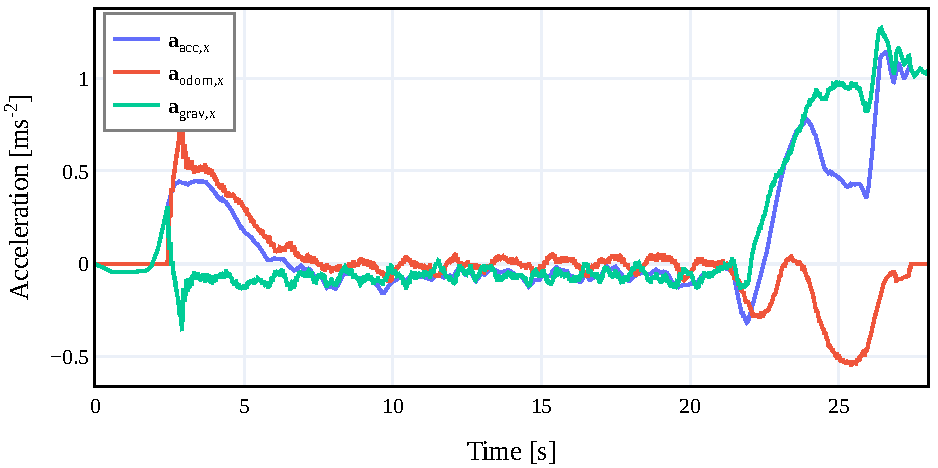
\includegraphics[width=.9\linewidth]{imu_odometer_acc.pdf}
	\caption[Acceleration from \gls{imu} and odometer]{Measured acceleration in x-direction by the \gls{imu} and acceleration derived from the wheel speed measurements and the difference between both}
	\label{fig:imu_odometer_acc}
\end{figure}
The resulting angle from the acceleration can be seen in \cref{fig:imu_odometer_angle}.
The reference is taken from the orientation estimation of the \texttt{hdl\_graph\_slam} package, which uses the \gls{lidar} data.
It can be seen that the gravity method improves the estimation accuracy significantly, compared to when only using the accelerometer data.
Especially the angle at the start and on the ramp is more accurately described when adding the odometer data to the accelerometer data for the calculation.
But it can also be seen that the time synchronization between both signals is important, as seen in during the initial acceleration phase.
Here, the subtraction leads to a negative value, which neither sensor had measured.\\
\begin{figure}[htbp]
	\centering
	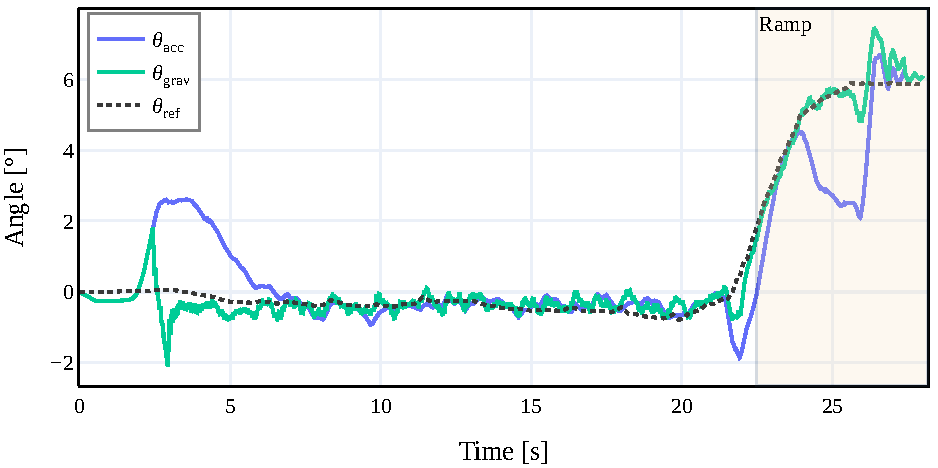
\includegraphics[width=.9\linewidth]{imu_odometer_angle.pdf}
	\caption[Gravity method]{Pitch angle estimation using only the accelerometer compared to the gravity method, which additionally uses the wheel speed measurements}
	\label{fig:imu_odometer_angle}
\end{figure}
Another way to improve the estimation is using a complementary filter, as shown in \cref{fig:imu_raw_compl_angle}.
The complementary filter uses the estimation of the gyroscope measurements and corrects them using the accelerometer measurements to prevent drift.
It can be seen that the estimation using the complementary filter closely follows the reference except for the \dots between the two ramps.
Also, it has no offset at the end, unlike the estimation from the gyroscope data.\\
Other methods of the same ride are shown in \cref{fig:imu_grav_compl_angle}.
The gravity method reduces the spikes of the raw accelerometer estimation, but introduces some new errors due to the odometer readings being slightly shifted in time in regard to the accelerometer readings.
The gravity complementary filter which fuses the estimation from the gravity method instead of only the accelerometer data together with the gyroscope data achieves the best results.
The filer gain could be reduced such that the estimation of the gravity method can be trusted more because it peaks less.
This makes the estimation more responsive to changes.
\begin{figure}[htb]
	\centering
	\begin{subfigure}{1\textwidth}
		\centering
		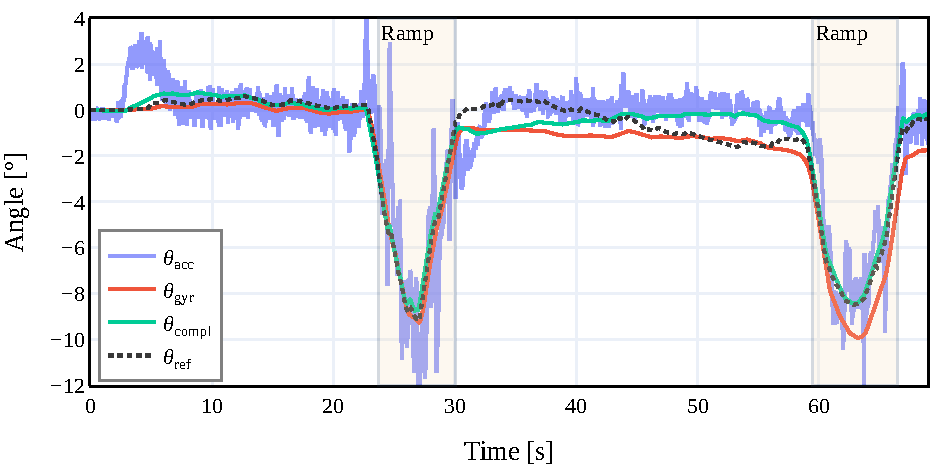
\includegraphics[width=0.9\linewidth]{imu_raw_compl_angle.pdf}
		\caption{Pitch angle estimation using the complementary filter compared to using the raw measurements}
		\label{fig:imu_raw_compl_angle}
	\end{subfigure}
	
	% \bigskip
	\begin{subfigure}{1\textwidth}
		\centering
		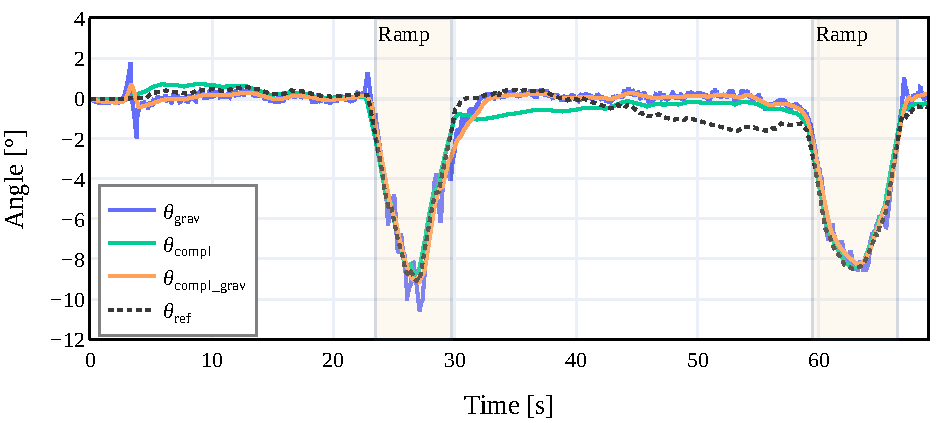
\includegraphics[width=0.9\linewidth]{imu_grav_compl_angle.pdf}
		\caption{Pitch angle estimation comparison of the other methods}
		\label{fig:imu_grav_compl_angle}
	\end{subfigure}
	\caption{Comparison of different methods to estimate the pitch angle}
\end{figure}
\itodo{Describe results shown in table}
\iimprov{Maybe mark best result for each column}
\begin{table}[htbp]
	\centering
	\caption{Performance measures up ZED \gls{imu}}
	\label{tab:eval_table_imu_up}
	\begin{tabular}[t]{ccccccc}
		\toprule
		\textbf{Properties}       & \multicolumn{3}{c}{\textbf{Ramp A}} & \multicolumn{3}{c}{\textbf{Ramp B}}                                                                                                     \\
		\midrule
		Mean($v$)                 & \multicolumn{3}{c}{3.7488}          & \multicolumn{3}{c}{3.9918}                                                                                                              \\
		Std($v$)                  & \multicolumn{3}{c}{1.9324}          & \multicolumn{3}{c}{1.8426}                                                                                                              \\
		Max($v$)                  & \multicolumn{3}{c}{5.3362}          & \multicolumn{3}{c}{5.3062}                                                                                                              \\
		Angle                     & \multicolumn{3}{c}{?}               & \multicolumn{3}{c}{?}                                                                                                                   \\
		\hline
		\textbf{Method}           & \textbf{RMSE} $[^\circ]$            & $\mathbf{R^2}$                      & \textbf{Angle} $[^\circ]$ & \textbf{RMSE} $[^\circ]$ & $\mathbf{R^2}$ & \textbf{Angle} $[^\circ]$ \\
		\cmidrule(lr){2-4}   \cmidrule(lr){5-7}
		Accelerometer             & 0.9478                              & 0.6508                              & 7.74                      & 0.6497                   & 0.7872         & 6.93                      \\
		Gyroscope                 & 0.8544                              & 0.7996                              & 4.78                      & 0.7910                   & 0.7797         & 4.34                      \\
		Acceleration method       & 0.4422                              & 0.9391                              & 7.95                      & 0.3499                   & 0.9555         & 7.06                      \\
		Complementary filter      & 0.6693                              & 0.8731                              & 4.96                      & 0.4514                   & 0.9307         & 4.92                      \\
		Complementary filter grav & $\mathbf{0.4113}$                   & 0.9619                              & 6.54                      & 0.2786                   & 0.9744         & 6.55                      \\
		\bottomrule
	\end{tabular}
\end{table}
\begin{table}[htbp]
	\centering
	\caption{Performance measures down ZED \gls{imu}}
	\label{tab:eval_table_imu_down}
	\begin{tabular}[t]{ccccccc}
		\toprule
		\textbf{Properties}       & \multicolumn{3}{c}{\textbf{Ramp C}} & \multicolumn{3}{c}{\textbf{Ramp A}}                                                                                                     \\
		\midrule
		Mean($v$)                 & \multicolumn{3}{c}{4.8088}          & \multicolumn{3}{c}{5.2509}                                                                                                              \\
		Std($v$)                  & \multicolumn{3}{c}{2.0341}          & \multicolumn{3}{c}{0.7972}                                                                                                              \\
		Max($v$)                  & \multicolumn{3}{c}{8.3662}          & \multicolumn{3}{c}{6.9711}                                                                                                              \\
		Angle                     & \multicolumn{3}{c}?                 & \multicolumn{3}{c}?                                                                                                                     \\
		\hline
		\textbf{Method}           & \textbf{RMSE} $[^\circ]$            & $\mathbf{R^2}$                      & \textbf{Angle} $[^\circ]$ & \textbf{RMSE} $[^\circ]$ & $\mathbf{R^2}$ & \textbf{Angle} $[^\circ]$ \\
		\cmidrule(lr){2-4}   \cmidrule(lr){5-7}
		Accelerometer             & 0.9417                              & 0.7065                              & -11.60                    & 1.0047                   & 0.7007         & -8.70                     \\
		Gyroscope                 & 0.3017                              & 0.9751                              & -9.21                     & 0.8147                   & 0.8470         & -9.92                     \\
		Acceleration method       & 0.3982                              & 0.9515                              & -10.18                    & 0.7200                   & 0.8752         & -8.43                     \\
		Complementary filter      & 0.2109                              & 0.9843                              & -9.03                     & 0.5525                   & 0.9356         & -9.22                     \\
		Complementary filter grav & 0.3490                              & 0.9653                              & -8.88                     & 0.6778                   & 0.8896         & -8.16                     \\
		\bottomrule
	\end{tabular}
\end{table}
\missingfigure{Plot of different compl gains}
\subsection{Ramp properties estimation}
\iquest{Ramp angle estimation already discussed in table or not?}
The measuring of the length of the ramp works well when the odometer readings are available.
The car velocity can then be integrated to get the travelled distance along the x-axis.
Without the odometer data it is more difficult, but still possible by using the accelerometer data.
By integrating the accelerometer data ... the velocity and another integration leads to the travelled distance.

\missingfigure{Plot of problem of distance estimation using only accelerometer (initial acc is bad)}
\todoin{\begin{itemize}
		\item Tune parameters
		\item Add distance measurement (for full drives)
		\item Ramp A = uc2s, Ramp B = us2c, Ramp C = dd2r, Ramp D = ds2c
	\end{itemize}}
\iquest{What about other \gls{imu}?}
\isug{Show results of other \gls{imu} at beginning (e.g. a plot) and say that the better one has been used from here on}



\section{Ramp detection (\glsentryshort{lidar} and camera)}
\subsection{\glsentryshort{lidar}}
The \gls{lidar} is used to detect if a ramp is visible, track the position to the ramp as well as to estimate the angle and width of the ramp.
Due to the setup it was only possible to mount one \gls{lidar} at a time.
To get the best possible results the \gls{lidar} with the best resolution, especially in vertical direction, should be used.
A comparison of the resolution of the two \glspl{lidar} can be seen in \cref{fig:lidar_resolution_eval}.
\begin{figure}[htbp]
	\centering
	\begin{subfigure}{1\textwidth}
		\centering
		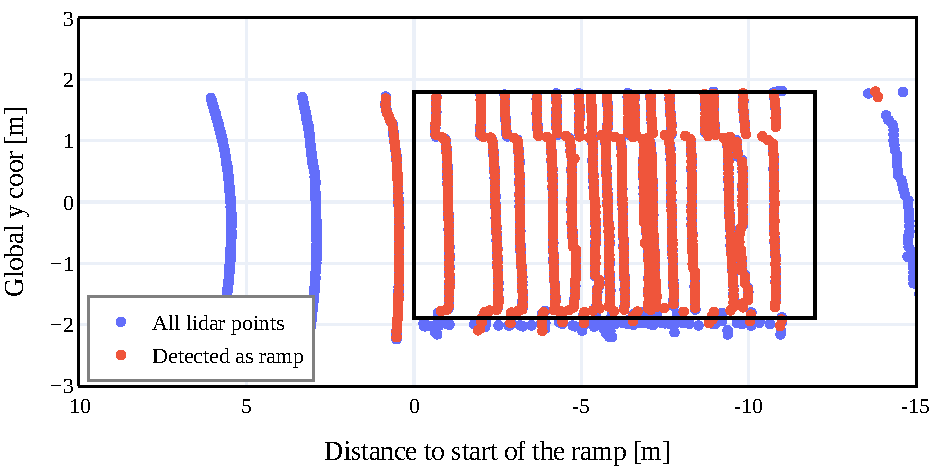
\includegraphics[width=.9\linewidth]{lidar_resolution_velodyne_eval.pdf}
		\caption{Velodyne}
		\label{fig:lidar_resolution_velodyne_eval}
	\end{subfigure}
	
	\begin{subfigure}{1\textwidth}
		\centering
		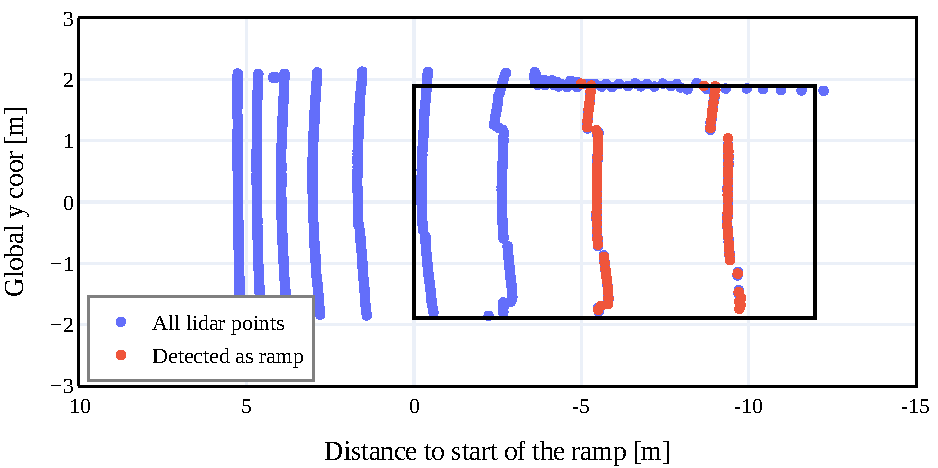
\includegraphics[width=.9\linewidth]{lidar_resolution_robos_eval.pdf}
		\caption{Robosense}
		\label{fig:lidar_resolution_robos_eval}
	\end{subfigure}
	\caption{Resolution comparison of the two \glspl{lidar}. The ramp region is framed in black. The Velodyne \gls{lidar} has a higher resolution.}
	\label{fig:lidar_resolution_eval}
\end{figure}
Here, a top-down view on the ramp of the points measured by the \gls{lidar} at a distance of \SI{7}{\metre} to the ramp is shown.
The blue points visualize all the points which were visible to the ramp detection algorithm after the downsampling and pass through filter has been applied.
The points marked red symbolize the points that were then detected as part of the ramp by the algorithm.
The ramp region is framed in black and was drawn manually by visually inspecting the by the \texttt{hdl\_graph\_slam} package generated point cloud.
The Velodyne \gls{lidar}, shown in \cref{fig:lidar_resolution_velodyne_eval}, provides many more lines compared to the Robosense, shown in \cref{fig:lidar_resolution_robos_eval}.
Hence, only the results produced using the Velodyne \gls{lidar} will be discussed from here on.\\
The detection rate is evaluated by using the number of \glspl{tp} and \glspl{fp}.
A frame is labeled as \gls{tp} if the ramp is visible, the algorithm detected a ramp and at least 50\% of the detected points lie inside the ramp region.
Analogously, a frame is classified as \gls{fp}, when a ramp was detected even though it was not visible or if less than 50\% of the detected points lie inside the ramp region.\\
The true distance to the ramp is measured by calculating the distance from the car's current position, which is provided by the \texttt{hdl\_graph\_slam} package, to the beginning of the ramp.
This value is used to evaluate performance of the tracking algorithm, by calculating the \gls{rmse} between this ground truth value and the estimated value.
The \gls{rmse} is also used to evaluate the accuracy of the angle and width estimation.
The estimated values are compared to values measured in the point cloud.\\
Since the resolution improves the closer the car gets to the ramp, the evaluation is divided into distance intervals of \SI{5}{\metre} of length.
The results for three different drives are shown in \cref{tab:eval_table_lidar}.
Each drive started about \SI{30}{\metre} from the ramp.
It can be seen that the detection works very well if the distance to the ramp is \SI{20}{\metre} or less.
For the ramp C? it can be seen, that the detection is only reliable when the car is less than \SI{15}{\metre} away from the ramp.
This can be explained by the taken path during the recording, which was started at an offset in y-direction to the ramp.
Due to the passthrough filter the ramp was thus not visible for the algorithm.\\
\todoin{\begin{itemize}
		\item Run script again, with correct true values (ramp angle and width)
		\item Right now same width and angle assumed for all ramps (and val is also wrong)
	\end{itemize}}
\iquest{Should TP and FP be replaced by precision and recall?}
\begin{table}[htbp]
	\centering
	\caption{Performance evaluation}
	\label{tab:eval_table_lidar}
	\begin{tabular}[t]{cccccccc}
		\toprule
		\textbf{Ramp}          & \textbf{Distance}        & \textbf{Frames} & \textbf{TP \%} & \textbf{FP \%} & $\textbf{RMSE}_d$  & $\textbf{RMSE}_w$ & $\textbf{RMSE}_\theta$ \\
		\midrule
		\multirow{6}{*}{u c2s} & \SIrange{0}{5}{\metre}   & 116             & 100.00\%       & 0.00\%         & \SI{0.73}{\metre}  & \SI{0.03}{\metre} & \SI{0.31}{\degree}     \\
		                       & \SIrange{5}{10}{\metre}  & 117             & 100.00\%       & 0.00\%         & \SI{0.73}{\metre}  & \SI{0.04}{\metre} & \SI{0.30}{\degree}     \\
		                       & \SIrange{10}{15}{\metre} & 116             & 100.00\%       & 0.00\%         & \SI{0.77}{\metre}  & \SI{0.07}{\metre} & \SI{0.34}{\degree}     \\
		                       & \SIrange{15}{20}{\metre} & 123             & 100.00\%       & 0.00\%         & \SI{1.07}{\metre}  & \SI{0.05}{\metre} & \SI{0.27}{\degree}     \\
		                       & \SIrange{20}{25}{\metre} & 140             & 99.23\%        & 0.00\%         & \SI{2.06}{\metre}  & \SI{0.12}{\metre} & \SI{0.65}{\degree}     \\
		                       & \SIrange{25}{30}{\metre} & 50              & 59.78\%        & 0.00\%         & \SI{1.66}{\metre}  & \SI{0.25}{\metre} & \SI{1.79}{\degree}     \\
		\hline
		\multirow{6}{*}{u s2c} & \SIrange{0}{5}{\metre}   & 62              & 100.00\%       & 0.00\%         & \SI{0.75}{\metre}  & \SI{0.02}{\metre} & \SI{0.52}{\degree}     \\
		                       & \SIrange{5}{10}{\metre}  & 62              & 100.00\%       & 0.00\%         & \SI{0.84}{\metre}  & \SI{0.02}{\metre} & \SI{0.53}{\degree}     \\
		                       & \SIrange{10}{15}{\metre} & 59              & 100.00\%       & 0.00\%         & \SI{0.89}{\metre}  & \SI{0.02}{\metre} & \SI{0.51}{\degree}     \\
		                       & \SIrange{15}{20}{\metre} & 61              & 97.92\%        & 2.08\%         & \SI{2.75}{\metre}  & \SI{0.02}{\metre} & \SI{0.68}{\degree}     \\
		                       & \SIrange{20}{25}{\metre} & 61              & 97.83\%        & 2.17\%         & \SI{3.69}{\metre}  & \SI{0.12}{\metre} & \SI{0.90}{\degree}     \\
		                       & \SIrange{25}{30}{\metre} & 59              & 42.75\%        & 0.00\%         & \SI{2.36}{\metre}  & \SI{0.90}{\metre} & \SI{1.82}{\degree}     \\
		\hline
		\multirow{6}{*}{u d2e} & \SIrange{0}{5}{\metre}   & 21              & 100.00\%       & 0.00\%         & \SI{0.94}{\metre}  & \SI{0.05}{\metre} & \SI{0.64}{\degree}     \\
		                       & \SIrange{5}{10}{\metre}  & 23              & 100.00\%       & 0.00\%         & \SI{0.79}{\metre}  & \SI{0.11}{\metre} & \SI{0.50}{\degree}     \\
		                       & \SIrange{10}{15}{\metre} & 28              & 100.00\%       & 0.00\%         & \SI{0.75}{\metre}  & \SI{0.10}{\metre} & \SI{0.44}{\degree}     \\
		                       & \SIrange{15}{20}{\metre} & 27              & 37.04\%        & 3.70\%         & \SI{2.59}{\metre}  & \SI{0.18}{\metre} & \SI{1.11}{\degree}     \\
		                       & \SIrange{20}{25}{\metre} & 29              & 0.00\%         & 3.45\%         & \SI{19.83}{\metre} & \SI{0.04}{\metre} & \SI{3.28}{\degree}     \\
		                       & \SIrange{25}{30}{\metre} & 28              & 10.71\%        & 0.00\%         & \SI{1.87}{\metre}  & \SI{0.25}{\metre} & \SI{1.91}{\degree}     \\
		\bottomrule
	\end{tabular}
\end{table}
The estimated ramp properties and distance to the ramp for one exemplary ride are shown in \cref{fig:lidar_eval}.
In \cref{fig:lidar_distance_eval} the estimated distance is shown in comparison to the reference distance provided by the \texttt{hdl\_graph\_slam} package.
The error reduces when the car is closer to the ramp.
Interestingly the value of the estimated distance seems to hold itself for several \si{\metre}.
This is most probably due to the vertical resolution of the \gls{lidar}.
Because the vertical resolution is not linear, the most lines are centered around the middle of the opening angle of the \gls{lidar}, which is -\ang{5} for the Velodyne.
Hence, only few lines fall into the region at the start of the ramp.
The distance to the ramp is calculated by measuring the distance from the car to the $n$ closest points which have been identified as part of the ramp.
Therefore, the distance can only be updated if a line which has previously hit the ground now hits the ramp.\\
Fig. \ref{fig:lidar_angle_eval} shows the difference between the estimated angle and the HOW measured angle.
It can be seen that the estimation varies by about \ang{1} if the distance is less than \SI{20}{\metre}.
The angle is almost exclusively underestimated (OR OVER?), which could be due to the fact that the measurement was wrong.\\
The estimated width at different distances to the ramp can be seen in \cref{fig:lidar_width_eval}.
The error is very small compared to the tracking error and lies in the order of \SI{10}{\cm}.
This is because the horizontal resolution is significantly better than the vertical resolution.
Note that the estimated width is the width of the whole ramp and not only the width of the drivable part.\\
\begin{figure}[htbp]
	\centering
	\begin{subfigure}{1\textwidth}
		\centering
		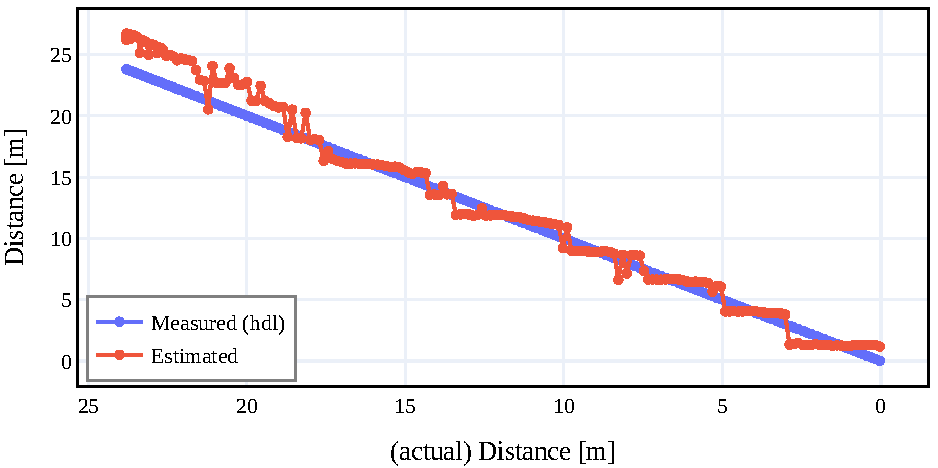
\includegraphics[width=.9\linewidth]{lidar_distance_eval.pdf}
		\caption{Distance to the ramp}
		\label{fig:lidar_distance_eval}
	\end{subfigure}
	
	\begin{subfigure}{1\textwidth}
		\centering
		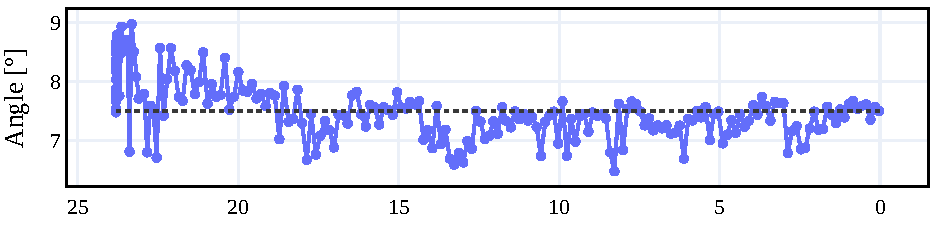
\includegraphics[width=.9\linewidth]{lidar_angle_eval.pdf}
		\caption{Angle of the ramp}
		\label{fig:lidar_angle_eval}
	\end{subfigure}
	
	\begin{subfigure}{1\textwidth}
		\centering
		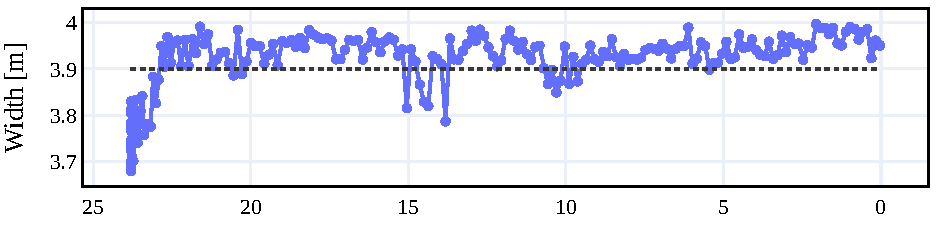
\includegraphics[width=.9\linewidth]{lidar_width_eval.pdf}
		\caption{Width of the ramp}
		\label{fig:lidar_width_eval}
	\end{subfigure}
	\caption{Estimated ramp properties and tracking of the ramp over ? using Velodyne}
	\label{fig:lidar_eval}
\end{figure}
An visualization of the detection algorithm can be seen in \cref{fig:points_projection}.
Here, the point cloud generated by the \gls{lidar} is projected onto to the camera image.
The quality of the projection depends on the accuracy of the measured translation and orientation difference between both sensors.
It can be seen that it is not perfect, e.g. the points do not quite match the camera image at the left pillar or the pipe on the ceiling.
Nonetheless it gives a good indication of what the \gls{lidar} actually sees.
The coloring of the point indicates the distance from the \gls{lidar} to the points.
Objects far away are marked by yellow points and nearby objects by blue points.
The green points were identified as part of the ramp by the algorithm.
It mostly fits the actual ramp very well.
The previously mentioned problem of the vertical resolution is clearly visible here.
While the density of the laser lines is sufficient in the ramp region, the start of the ramp and especially the ground is covered by very few lines.
This makes the precise tracking of the distance to the ramp difficult.
\begin{figure}[htbp]
	\centering
	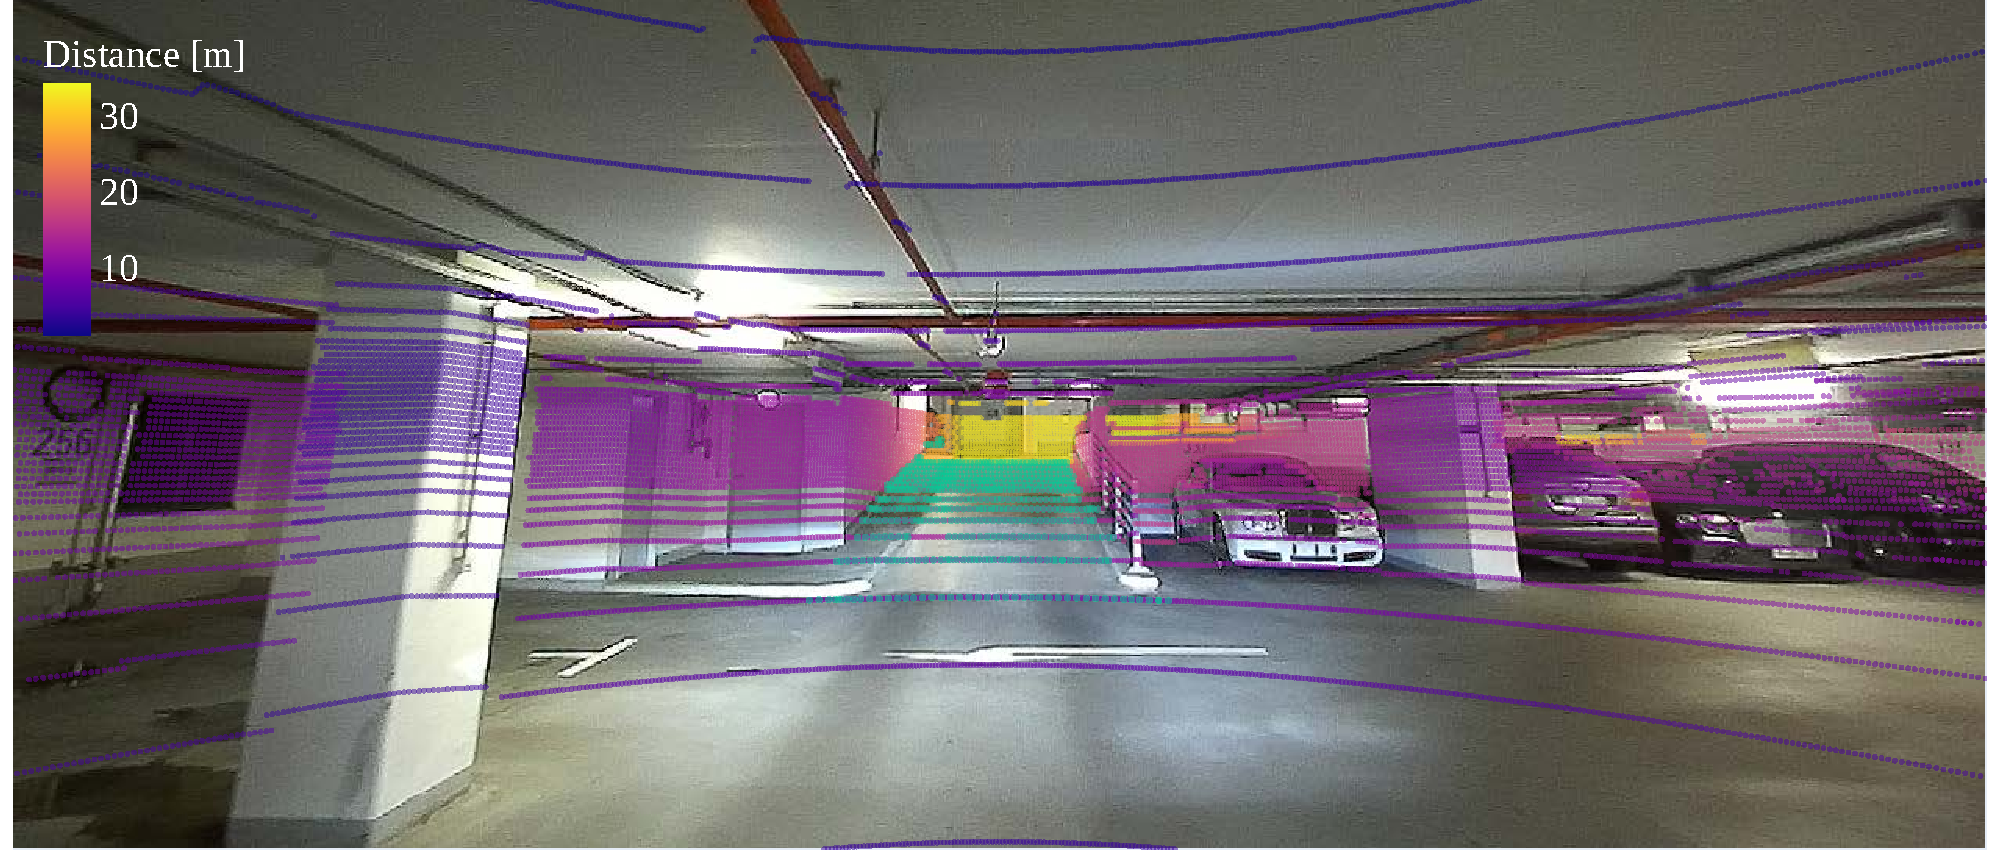
\includegraphics[width=1\linewidth]{points_projection.pdf}
	\caption{Lidar points projected into the camera image. The green points were identified as part of a ramp.}
	\label{fig:points_projection}
\end{figure}



\subsection{Camera}
The camera was used to detect the ramp and mask the region.
\begin{figure}[htbp]
	\centering
	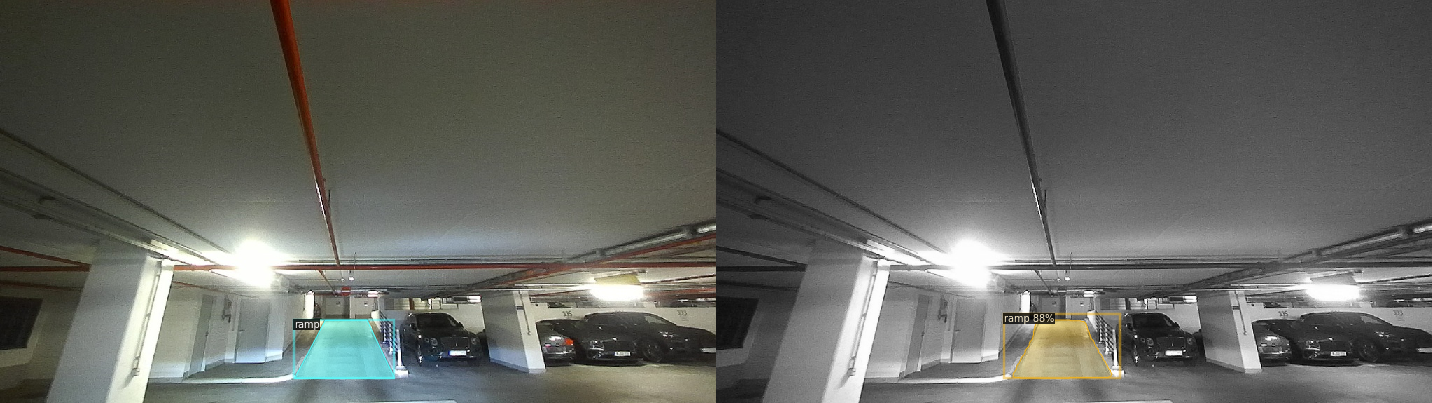
\includegraphics[width=1\linewidth]{camera_detection_compare}
	\caption{Machine learning}
	\label{fig:camera_detection_compare}
\end{figure}
\begin{equation}
	\text{Precision} = \frac{TP}{TP+FP}
\end{equation}
\begin{equation}
	\text{Recall} = \frac{TP}{TP+FN}
\end{equation}
$TP$ is the number of true positives, $FP$ is the number of false positives and $FN$ is the number of false negatives.
So the precision gives information about how accurate the predictions are and the recall gives information about how much of the ground truth is detected.

The \gls{ap} is a detection evaluation metric used by the \gls{coco} dataset.
$\text{AP}_{50}$ means how many detections have been made with an \gls{iou} score of at least 50\%.
The \gls{iou} is defined as
\begin{equation}
	\text{\acrshort{iou}} = \frac{\text{Area of Overlap}}{\text{Area of Union}}.
\end{equation}
The area of overlap is defined as the intersection between the predicted and ground truth bounding box, and the area of union is the area of both boxes added together.
A perfect detection would have an \gls{iou} score of 1.
Since selecting a meaningful threshold for the \gls{ap} score depends on the dataset, an average score \gls{map} is used.
The \gls{map} scores is the average over multiple \gls{iou} thresholds for all the different classes.
It is calculated by averaging all \gls{ap} scores in the range of 50\% to 95\% with a step size of 5\%, meaning that the average of 10 different values is used.

% \begin{table}
% 	\centering
% 	\caption[Detection evaluation]{bla}
% 	\label{tab:detection_eval}
% 	\begin{tabular}[htb]{ccccccc}
% 		\toprule
% 		\textbf{Epochs} & \textbf{LR} & \textbf{SR} & \textbf{Box mAP} & $\textbf{Box AP}_{75}$ & $\textbf{Mask mAP}$ & $\textbf{Mask AP}_\mathbf{75}$ \\
% 		\midrule
% 		1.0             & 0.025       & 128.0       & 55.8             & 79.4                   & 52.5                & 100.0                          \\
% 		1.0             & 0.025       & 512.0       & 81.1             & 86.1                   & 100.0               & 100.0                          \\
% 		\bottomrule
% 	\end{tabular}
% \end{table}

\begin{table}
	\centering
	\caption[Detection evaluation]{bla}
	\label{tab:detection_eval1}
	\begin{tabular}[H!]{ccccccc}
		\toprule
		\textbf{Epochs} & \textbf{LR} & \textbf{SR} & \textbf{Box mAP} & \textbf{Mask mAP} \\
		\midrule
		1               & 0.05        & 256         & 39.8             & 64.8              \\
		1               & 0.01        & 256         & 73.1             & 84.7              \\
		1               & 0.005       & 256         & 78.4             & 85.9              \\
		1               & 0.001       & 256         & 82.1             & 89.7              \\
		2               & 0.05        & 256         & 58.0             & 74.3              \\
		2               & 0.01        & 256         & 83.1             & 87.2              \\
		2               & 0.005       & 256         & 83.9             & 90.2              \\
		2               & 0.001       & 256         & 85.3             & 89.5              \\
		\bottomrule
	\end{tabular}
\end{table}

\begin{table}
	\centering
	\caption[Detection evaluation]{bla}
	\label{tab:detection_eval}
	\begin{tabular}[H!]{ccccccc}
		\toprule
		\textbf{Epochs} & \textbf{LR} & \textbf{SR} & \textbf{Box mAP} & \textbf{Mask mAP} \\
		\midrule
		1               & 0.005       & 128         & 67.4             & 81.6              \\
		1               & 0.005       & 512         & 80.5             & 85.8              \\
		1               & 0.001       & 128         & 86.1             & 87.3              \\
		1               & 0.001       & 512         & 86.2             & 90.5              \\
		3               & 0.005       & 128         & 71.6             & 80.6              \\
		3               & 0.005       & 512         & 85.6             & 86.2              \\
		3               & 0.001       & 128         & 87.3             & 91.7              \\
		3               & 0.001       & 512         & 89.0             & 90.3              \\
		\bottomrule
	\end{tabular}
\end{table}